\documentclass[10pt]{article}
\usepackage{graphicx}  % For including the image
\usepackage{geometry}  % For setting margins
\usepackage{fancyhdr}  % Optional, for setting a persistent header/footer
\usepackage{enumitem} 
\usepackage{pgfgantt} 
\usepackage[table]{xcolor}  
\usepackage{colortbl}      
\usepackage[document]{ragged2e}

\geometry{a4paper, margin=0.8in}

% --- Custom Footer Setup ---
\pagestyle{fancy}
\fancyhf{} % Clear headers/footers
\fancyfoot[L]{\thepage\ / Volume 1, 2025} 
\fancyfoot[R]{FIBO FRA333 – Kinematics Final Project}
\renewcommand{\headrulewidth}{0pt}
\renewcommand{\footrulewidth}{0.5pt}
% ---------------------------

\begin{document}

\noindent
\begin{tabular}{p{0.90\textwidth} c} 
    \parbox[t]{0.90\textwidth}{ 
        \raggedright 
        Institute of Field Robotics, King Mongkut's University of Technology Thonburi \\
        126 Pracha Uthit Rd, Bang Mot, Thung Khru, Bangkok, Thailand 10140 \\
        Senior Thesis FRAB (FIBO Robotics and Automation: Bachelor) \\
        Copyright $\copyright$ 2021 by FIBO
        \vspace{0.5cm}
    }
    & 
    \raisebox{-1.4cm}
    {
        
\includegraphics[width=0.7in, keepaspectratio]{img/fibo_logo.png}
    }
\end{tabular}

\noindent
\rule{\textwidth}{1pt}

\vspace{0.4cm}
\noindent
\Large {\textbf{A study of Torque-Control system on UR5 for the drawing task}}

\noindent
\rule{\textwidth}{0.3pt}

\begin{minipage}[t]{0.40\textwidth}
    \raggedright
    \normalsize
    Jirattanun Leeudomwong, 66340500009 \\
    Bharut Aursudkit, 66340500040 \\
    Nuttapruet Puttiwarodom, 66340500018 \\
\end{minipage}
\hfill
\vline
\begin{minipage}[t]{0.60\textwidth}
    \raggedright
    \normalsize
    \begin{quote}
        \textbf{Abstract} \\
        Industrial robot manipulators have countless applications nowadays. One of the basic tasks to test the accuracy of a robot manipulator is to perform a drawing task, which can be done with only position control alone. This project focuses on using a UR5 industrial robot manipulator to perform the drawing task. The challenge this project represents is controlling the force between the pen (end-effector) and the canvas using torque control while following a trajectory generated by the image processing method. This project is running on Gazebo Ignition physics simulation and using ROS2 as a middleware.
        \vspace{0.5cm}

        \textbf{Keywords: Torque control, Dynamics model, Trajectory generation, Image processing, Edge detection, ROS2, Physic simulation}
    \end{quote}
\end{minipage}

\vspace{0.4cm}
\noindent
\rule{\textwidth}{1pt}

\linespread{1.5} 
% ------------------- context zone ------------------- 
\vspace{0.2cm}
\noindent
\large
\textbf{1. Introduction} \\
\textbf{1.1 Objective}  \\
\normalsize
\begin{enumerate}[nosep, itemsep=-2pt] 
    \item To develop the UR5 industrial robot manipulator to perform the drawing task in Gazebo Ignition physics simulation. 
    \item Design and implement a torque control system that can follow position, velocity, and torque trajectories.
    \item To create a trajectory generation process that can generate a path from any input image.
\end{enumerate}
  
\vspace{8pt}
\noindent
\large 
\textbf{1.2 Scope of the study} \\ 
\normalsize
\begin{enumerate}[nosep, itemsep=-2pt] 
    \item This project is conducted and tested only in the Gazebo Ignition physics simulation environment using the ROS2 middleware; real-world implementation is not included.
    \item This project only covers drawing task with 1 fixed drawing plain and not coverage pen changing, drawing at multiple plains, or other additional tasks.
\end{enumerate}

\newpage

\large
\noindent
\textbf{2. Review of the literature} \\
\normalsize
\indent Controlling the torque is important to control the motion of a manipulator while still respecting joint limits. Del Prete (2017) provides a method for torque control that ensures feasible future trajectories while accounting for constraints in position, velocity, and torque. It is shown to be computationally efficient and applicable for high-frequency real-time control through numerical simulations. The method directly relates to a UR5 drawing task in which the joint torque and acceleration limits must be respected while the end-effector tracks the desired trajectories.

\indent Belalia and colleagues (2024) suggest a vision-based approach for robotic trajectory tracking that uses convolutional neural networks (CNN) and Spline3 interpolation. The CNN tracks object locations from sequences of images, and the information is applied to produce smooth trajectories "with high accuracy and minimal oscillation." While their solution has an improvement in accuracy, the CNN approach is excessively complicated for this project, and simpler image recognition techniques can achieve adequate accuracy for end-effector trajectory generation of the UR5 drawing task.

\indent Moreover, simulation platforms, like Gazebo Ignition and ROS2, allow the robot control systems to be tested prior to implementation in the real world, while being safe and flexible enough to test torque control and trajectory tracking, without damaging the robot or workspace. Simulation is important for any task involving contact forces (e.g., the UR5 drawing task), where position and force must be controlled simultaneously.

\indent While there have been advancements in torque control, vision-based trajectory generation, and simulation, not many have examined these together in terms of specific tasks such as robotic drawing. This project aims to fill that gap and combines torque control and image-based trajectory generation in simulation to allow for the precision of end-effector movement while handling force and positional constraints.

\large
\noindent
\textbf{3. Related knowledge with FRA333} \\
\normalsize
\begin{enumerate}[nosep, itemsep=-2pt]
    \item Forward Kinematics 
    \item Inverse Kinematics
    \item Differential Kinematics
    \item Dynamics
    \item Trajectory generation
\end{enumerate}

\newpage

\large
\noindent
\textbf{4. System diagram} \\
\normalsize
\indent
\begin{figure}[h]
    \centering
    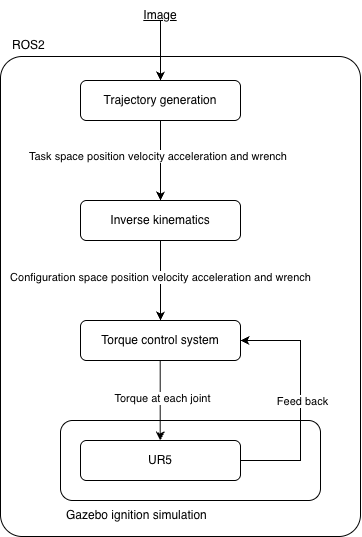
\includegraphics[width=5cm,keepaspectratio]{img/system_diagram.png}
    \caption{Project system diagram}
    \label{fig:system diagram} 
\end{figure}
\vspace*{-0.5\baselineskip} 
\begin{enumerate}[itemsep=-2pt]
    \item \textbf{Trajectory generation}: 
    The trajectory will generate the task space position, velocity, and acceleration based on the input image. This trajectory can not only specify the desired position for the robot to perform the drawing, but also assign the force between the pen (end-effector) and the canvas, known as a wrench, allowing the robot to draw with varying pressure on the same canvas. 
    \item \textbf{Inverse Kinematics}: 
    The control system requires the configuration space position, velocity, and acceleration to control the joint. However, the trajectory generation process yields the task space position, velocity, and acceleration. Inverse Kinematics helps map the task space position, velocity, and acceleration into configuration space.
    \item \textbf{Torque control system}:
    The control system is responsible for making the UR5 follow the trajectory. The specific method that allows the robot to follow the position, velocity, acceleration, and wrench trajectory without relying on multiple, separate controllers is Hybrid Motion-Force Control.
    \begin{equation}
       \tau = M(q)\ddot{q}_r + C(\dot{q}, q) + g(q) + J^T(q)W
    \end{equation}
    \begin{equation}
        \ddot{q}_r = \ddot{q}_d + K_d(\dot{q}_d - \dot{q}) + K_p (q_d - q)
    \end{equation}
    \vspace{-10pt}
    where:
    \begin{center}
    \begin{tabular}{c c p{10cm}}
        $\mathbf{\tau}$ & is & the vector of joint torque inputs (Nm). \\
        $\mathbf{M}(q)$ & is & the robot mass matrix (or inertia matrix). \\
        $\mathbf{C}(q, \dot{q})$ & is & the vector of Coriolis and centrifugal torques. \\
        $\mathbf{g}(q)$ & is & the vector of gravitational torques. \\
        $\ddot{q}_r$ & is & the required joint acceleration vector from PD control (2). \\
        $W$ & is & the wrench
    \end{tabular}
    \end{center}
    
    \item \textbf{UR5}: 
    To enable control and testing of the UR5, the Gazebo Ignition physics simulation is used to model the robot's actions and responses.
\end{enumerate}

\newpage

\large
\noindent
\textbf{5. Learning outcome} \\
\normalsize
\begin{enumerate}[nosep, itemsep=-2pt]
    \item To study a Torque-Control system design that is able to follow the position, velocity, acceleration, and wrench trajectory using a dynamics model. 
    \item To study and develop the process of trajectory generation from image processing.
    \item To study robot control and simulation using ROS2 and Gazebo Ignition.
\end{enumerate}

\large
\noindent
\textbf{6. Gantt chart} \\
\normalsize
\renewcommand{\figurename}{Table} %in norm package{pgfgantt} use figure,so I has change it!
\definecolor{ganttbar}{RGB}{200,200,200}  % Color for tasks Highlight
\begin{table}[h]
\centering
\begin{tabular}{|c|l|c|c|c|c|c|}
\hline
\textbf{No.} & \textbf{Task} & \textbf{Week 1} & \textbf{Week 2} & \textbf{Week 3} & \textbf{Week 4} & \textbf{Week 5} \\ \hline
1 & Literature & \cellcolor{ganttbar} &  &  &  &  \\ \hline
2 & System and Simulation setup & \cellcolor{ganttbar} &  &  &  &  \\ \hline
3 & Inverse Kinematics &  & \cellcolor{ganttbar} &  &  &  \\ \hline
4 & Torque Control &  & \cellcolor{ganttbar} & \cellcolor{ganttbar}  &  &  \\ \hline
5 & Trajectory Generation &  & \cellcolor{ganttbar} & \cellcolor{ganttbar}  &  &  \\ \hline
6 & Integration &  &  & \cellcolor{ganttbar} &  &  \\ \hline
7 & Testing &  &  &  & \cellcolor{ganttbar} &  \\ \hline
8 & Evaluation &  &  &  &  & \cellcolor{ganttbar} \\ \hline
\end{tabular}
\caption{Project Gantt Chart Summary (5 Weeks).}
\label{tab:gantt_excel}
\end{table}


\large
\noindent
\textbf{7. Reference} \\
\normalsize 
[1] A. Del Prete, “Joint Position and Velocity Bounds in Torque Control of Robot Manipulators,” *IEEE Robotics and Automation Letters*, vol. 3, no. 1, pp. 281–288, Jan. 2018. \\

[2] A. Belalia, S. Chouraqui, and M. Boussir, “Trajectory Tracking of a Robot Arm Using Image Sequences,” *Journal of Robotics and Computer Vision*, 2024. \\

\end{document}